\documentclass[aspectratio=169]{beamer}
\usetheme{default}
\usepackage{slidesonnet}
\usepackage{tikz}
\usetikzlibrary{arrows.meta, positioning}
\title{Pipeline and Beamer}
\begin{document}

\begin{frame}{The slideSonnet Pipeline}
  \begin{center}
  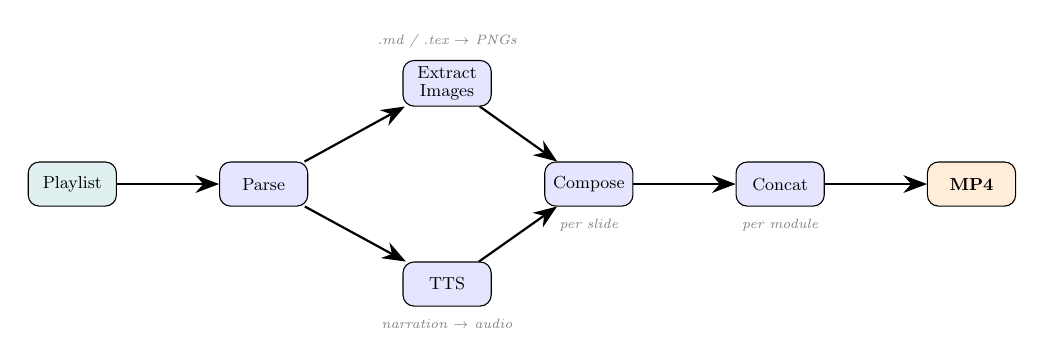
\begin{tikzpicture}[scale=0.7, every node/.style={scale=0.7},
    node distance=1.0cm and 1.3cm,
    box/.style={rectangle, draw, rounded corners, minimum height=0.8cm,
                minimum width=1.6cm, align=center, font=\small},
    src/.style={box, fill=teal!12},
    proc/.style={box, fill=blue!10},
    result/.style={box, fill=orange!15},
    arr/.style={-{Stealth[length=3mm]}, thick},
    note/.style={font=\scriptsize\itshape, text=gray}
  ]
    \node[src] (play) {Playlist};
    \node[proc, right=of play] (parse) {Parse};
    \node[proc, above right=0.7cm and 1.2cm of parse] (img) {Extract\\[-2pt]Images};
    \node[proc, below right=0.7cm and 1.2cm of parse] (tts) {TTS};
    \node[proc, right=3cm of parse] (comp) {Compose};
    \node[proc, right=of comp] (cat) {Concat};
    \node[result, right=of cat] (mp4) {\textbf{MP4}};

    \draw[arr] (play) -- (parse);
    \draw[arr] (parse) -- (img);
    \draw[arr] (parse) -- (tts);
    \draw[arr] (img) -- (comp);
    \draw[arr] (tts) -- (comp);
    \draw[arr] (comp) -- (cat);
    \draw[arr] (cat) -- (mp4);

    \node[note, above=2pt of img] {.md / .tex $\to$ PNGs};
    \node[note, below=2pt of tts] {narration $\to$ audio};
    \node[note, below=2pt of comp] {per slide};
    \node[note, below=2pt of cat] {per module};
  \end{tikzpicture}
  \end{center}

  \say{This diagram shows the slideSonnet pipeline. The playlist is parsed to extract slides and narration. These fan out into two parallel paths: image extraction and speech synthesis. The compose step merges each slide image with its audio, then concat joins the segments per module into the final MP4.}
\end{frame}

\begin{frame}{LaTeX Math}
  Euler's identity:
  \[ e^{i\pi} + 1 = 0 \]

  \vspace{0.5cm}
  The Cauchy--Schwarz inequality:
  \[ \left( \sum_{k=1}^{n} a_k b_k \right)^2
     \leq
     \left( \sum_{k=1}^{n} a_k^2 \right)
     \left( \sum_{k=1}^{n} b_k^2 \right) \]

  \say{Beamer excels at typesetting mathematics. Here we see Euler's identity and the Cauchy Schwarz inequality, rendered with full LaTeX quality.}
\end{frame}

\begin{frame}{Beamer Annotations}
  Beamer slides use LaTeX commands instead of HTML comments:

  \begin{itemize}
    \item \texttt{\textbackslash say\{narration text\}} \quad --- basic narration
    \say{In Beamer, you narrate slides with the backslash say command, followed by your text in curly braces.}
    \pause
    \item \texttt{\textbackslash say[voice=expert]\{text\}} \quad --- voice override
    \say[2]{You can pass optional parameters in square brackets, like voice equals expert, to change the voice for a specific slide.}
    \pause
    \item \texttt{\textbackslash nonarration} \quad --- silent slide
    \item \texttt{\textbackslash slidesonnetskip} \quad --- skip slide
    \say[3, voice=expert]{Backslash nonarration creates a pause with no speech, and backslash slidesonnetskip excludes a slide entirely. The same voices and pronunciation dictionaries apply across all module types.}
  \end{itemize}
\end{frame}

\begin{frame}{End of Beamer Section}
  \nonarration
\end{frame}

\end{document}
